% Tier 1 result: paired R/C ratios of the 16 alternating pairs, GitHub run 38502816475.
% Data: ../tier1_github_38502816475/verdict.json (primary.per_pair, secondary.per_pair).
% Source of tier1_result.pdf; build: pdflatex tier1_result.tex
\documentclass[border=6pt]{standalone}
\usepackage{pgfplots}
\pgfplotsset{compat=1.17}
\begin{document}
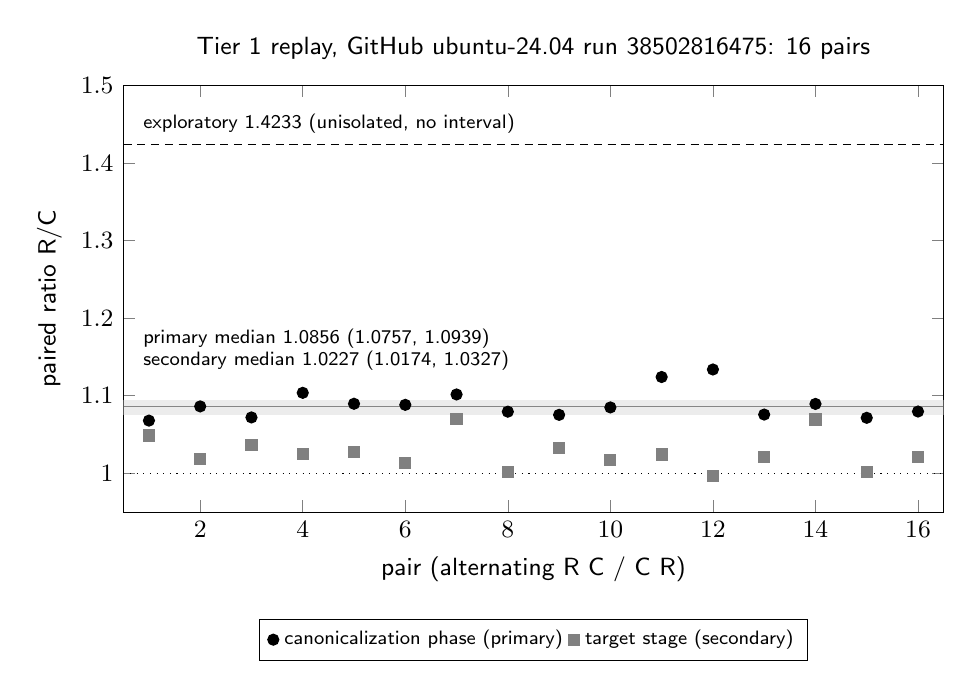
\begin{tikzpicture}[font=\sffamily\small]
\begin{axis}[width=12cm, height=7cm, xmin=0.5, xmax=16.5, ymin=0.95, ymax=1.5,
  xlabel={pair (alternating R C / C R)}, ylabel={paired ratio R/C},
  title={Tier 1 replay, GitHub ubuntu-24.04 run 38502816475: 16 pairs},
  title style={font=\sffamily\small}, legend style={at={(0.5,-0.25)}, anchor=north, legend columns=2, font=\sffamily\scriptsize}]
\addplot[only marks, mark=*, mark size=2pt] coordinates {(1,1.0679) (2,1.0862) (3,1.0720) (4,1.1037) (5,1.0896) (6,1.0882) (7,1.1016) (8,1.0794) (9,1.0753) (10,1.0849) (11,1.1241) (12,1.1338) (13,1.0757) (14,1.0894) (15,1.0715) (16,1.0796)};
\addplot[only marks, mark=square*, mark size=2pt, color=gray] coordinates {(1,1.0487) (2,1.0180) (3,1.0367) (4,1.0252) (5,1.0269) (6,1.0131) (7,1.0701) (8,1.0019) (9,1.0327) (10,1.0174) (11,1.0241) (12,0.9961) (13,1.0213) (14,1.0694) (15,1.0014) (16,1.0207)};
\draw[solid] (axis cs:0.5,1.0856) -- (axis cs:16.5,1.0856);
\fill[black!12, opacity=0.6] (axis cs:0.5,1.0757) rectangle (axis cs:16.5,1.0939);
\draw[densely dashed] (axis cs:0.5,1.4232676) -- (axis cs:16.5,1.4232676);
\draw[dotted] (axis cs:0.5,1) -- (axis cs:16.5,1);
\node[anchor=south west, font=\sffamily\scriptsize] at (axis cs:0.7,1.425) {exploratory 1.4233 (unisolated, no interval)};
\node[anchor=south west, font=\sffamily\scriptsize, align=left] at (axis cs:0.7,1.12) {primary median 1.0856 (1.0757, 1.0939)\\secondary median 1.0227 (1.0174, 1.0327)};
\legend{canonicalization phase (primary), target stage (secondary)}
\end{axis}
\end{tikzpicture}
\end{document}
